\section{The effect of phase relative velocity on the rheology of mono-disperse dilute emulsion}


In this section we make use of the \textit{hybrid model} to demonstrate how to derive the minimal set of equation intended to model deformable droplets in a buoyant emulsion. 

The preceding studies on the subject have intended to model the rheology of dilute emulsion of neutrally buoyant deformable droplets, in stokes regime \citep{goddard1967nonlinear,lhuillier1987phenomenology,maffettone1998equation}.
More recently, researcher have been trying to include inertial effect in these models \citet{raja2010inertial,mwasame2018macroscopic}. 
However, these studies have been conducted in the objective of determining the equivalent shear stress of a neutrally buoyant suspension, i.e. they study the mean stress $\bm{\sigma}(\textbf{E})$ due to an imposed flow gradient $\textbf{E}$ for a given microstructure. 
Therefore, to the knowledge of the author all preceding study disregards the impact of relative motion on the suspension rheology. 

In this application we therefore focus on the Rheological behavior of an inertial buoyant emulsion when the relative motion between phases $\textbf{U} = \textbf{u}_1 - \textbf{u}_2$ isn't null. 
This situation is present in most of the emulsion appearing in industrial processes. 
We seek therefore for an expression of the bulk stress of the form $\bm{\sigma}(\textbf{U},\textbf{E})$. 
Additionally, as it has been demonstrated by \citet{haber1971dynamics} the deformation of a droplet can lead to a lift force push the droplet outward a poiseuil flow.
It is therefor primordial to determine the averaged deformation of the drops. 

\subsubsection*{The spheroidal particle geometry}

For simplicity, and because it doesn't remove any of the arguments, we assume a spheroidal particle shape. 
Unlike \citet{goddard1967nonlinear,lhuillier1987phenomenology} and following \citet{maffettone1998equation,mwasame2017macroscopic} we describe the particle's shape with a second order dimensionless contravariant conformation tensor, $\textbf{C}_\alpha$.
\begin{figure}[h!]
    \centering
    \hfill
    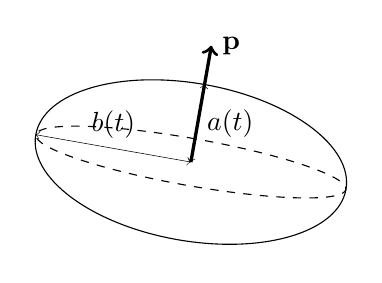
\begin{tikzpicture}[rotate=80]
        \draw(0,0) ellipse (1 cm and 2 cm);
        \draw[dashed](0,0) ellipse (0.3 cm and 2 cm);
        \draw[<->,very thin](0,0) --++ (1,0)node[midway,right]{$a(t)$};
        \draw[->,very thick](0,0) --++ (1.5,0)node[right]{$\textbf{p}$};
        \draw[<->,very thin](0,0) --++ (0,2)node[midway,above]{$b(t)$};
    \end{tikzpicture}
    \hfill
    \caption{Scheme of an  oblate spheroid oriented along the unit vector \textbf{p}.}
    \label{fig:scheme2}
\end{figure}
This tensor is defined such that its eigenvalues are the dimensionless square length of the semi-axis of the spheroid, such that $\textbf{C}_\alpha = a^2/r_0^2 \textbf{pp} + b^2 /r_0^2 (\textbf{I}-\textbf{pp})$ where $r$ is the radius of the sphere of same volume. 
This definition is convenient since it can be shown that $\textbf{C}_\alpha$ is equivalent to the Cauchy strain tensor well-defined in solid mechanics \citet{mwasame2017macroscopic}. 
Therefore, in a general coordinate system the point on the surface of the spheroid respect the equation, 
\begin{equation*}
    \textbf{r}\cdot\textbf{C}^{-1}\cdot\textbf{r} = r_0^2,
\end{equation*}
where $\textbf{C}$ is the inverse operator. 

Additionally, one can verify that the second order moment of mass of the particles is related to the conformation tensor through, $\textbf{M}_\alpha = \frac{m_\alpha  r_0^2}{5} \textbf{C}$. 
One can show that the constant volume constrain can be obtained by ensuring that $\text{det}(\textbf{C}) = (ab^2)^2 /(r_0^6) = 1$. 
It must be understood that at equilibrium the particle reach a spherical shape and therefore has $\textsc{C} = \textbf{I}$. 

\subsubsection*{The drop internal kinematic equation}



The evolution of $\textbf{C}_\alpha$ and $\bm\Gamma_\alpha$ will be described by the second moment of mass and first moment of momentum equation.
Consequently, we must reformulate the terms in \ref{eq:dt_M_alpha} and \ref{eq:dt_P_alpha} in terms of $\textbf{C}_\alpha$ and $\bm\Gamma_\alpha$. 
The integrals constitutive of these moments equations can be written, 
\begin{align}
    \intO{(\textbf{rw}_2^0 )_{ij}+ (\textbf{w}_2^0 \textbf{r})_{ij}} 
    = \textbf{C}_{\alpha,ik} \cdot \bm\Gamma_{\alpha,kj}
    +  \bm\Gamma_{\alpha,ki} \cdot \textbf{C}_{\alpha,jk}
    % +  \bm\Gamma_{\alpha,ij} + \bm\Gamma_{\alpha,ij}
    \\
    \intO{\rho_2 \textbf{w}_{2,i}^0\textbf{w}_{2,j}^0}
    = \frac{m_\alpha a^2}{5}
        \bm\Gamma_{\alpha,lj}\bm\Gamma_{\alpha,ki} \textbf{C}_{\alpha,kl} 
        % + \bm\Gamma_{\alpha,kj}\bm\Gamma_{\alpha,ki} 
        % + f_\textbf{ww}(\textbf{u}_\alpha,\textbf{C}_\alpha,\bm\Gamma_\alpha,\textbf{u}_1,\bm \Gamma_1,\phi_2)
        + \intO{\rho_2\textbf{w}^s_2\textbf{w}^s_2}
    \\
    \label{eq:sigma_2_def}
    \intO{\bm\sigma_{2,ij}^0}
    =
    % -\intO{p_2^0} \textbf{I}_{ij}
    \mu_2 v_\alpha (\bm\Gamma_{\alpha,ij} + \bm\Gamma_{\alpha,ij})
    + \mu_2 \intS{\textbf{w}^s_{2,i}\textbf{n}_{2,j}+ \textbf{w}^s_{2,j}\textbf{n}_{2,i}}
    + \textbf{I}_{ij}\intO{p_2^0} 
    \\
    \label{eq:sigma_I_def}
    \intS{\bm\sigma_{I,ij}^0}
    = \frac{2 \gamma v_\alpha }{a} \textbf{I}_{ij} - \frac{4 \gamma v_\alpha }{5 a} \textbf{C}_{\alpha,ij}
    +\mathcal(|\textbf{C}|^2)\\
    \intS{\textbf{r}\bm\sigma_1^0\cdot \textbf{n}_2}
    = 
    \frac{1}{2}\intS{(\textbf{r}\bm\sigma_1^0-\bm\sigma_1^0\textbf{r})\cdot \textbf{n}_2}
    + \frac{1}{2}\intS{(\textbf{r}\bm\sigma_1^0+\bm\sigma_1^0\textbf{r})\cdot \textbf{n}_2}
    % \textbf{M}(\textbf{u}_\alpha,\textbf{C}_\alpha,\bm\Gamma_\alpha,\textbf{u}_1,\bm \Gamma_1,\phi_2)
\end{align}
First, as discussed above only the deforming motion contribute to the symmetric part of the moment of momentum, we could therefore express it explicitly in terms of the particle unknown. 
Regarding the first moment of the surface tension, it has been computed analytically carrying a surface integral on the ellipsoidal surface of the droplet. 
Since, the droplets remain spheroidal under small deformation we choose to approximate $\intS{\bm\sigma_I^0}$ with its first order Taylor series in $\textbf{C}_\alpha$ without lost of generality.
Note that our expression of $\intS{\bm\sigma_I^0}$ is in agreement with \citet{lhuillier1987phenomenology} if one account for the slight difference of his definition of the deformation tensor which is half of $\textbf{C}_{\alpha}$. 
% in which our $\textbf{C}_\alpha$ is twice his, in the limit of small \textbf{C}_\alpha.
For the expression of $\intO{\rho_2 \textbf{w}_{2,i}^0\textbf{w}_{2,j}^0}$, $ \intO{\bm\sigma_{2,ij}^0}$ we had to introduce two unknown functions, $f_\textbf{ww}$, $f_{\bm{\sigma}}$, which vanish when $\textbf{w}^s_2 =0$. 
Therefore, these expressions are a sum of a function involving $\bm\Gamma_\alpha$ and an unknown part which depend on the parameters of the problem and need to be closed. 
The expression of $\intO{\rho_2 \textbf{w}_{2,i}^0\textbf{w}_{2,j}^0}$, $ \intO{\bm\sigma_{2,ij}^0}$ and $\intS{\textbf{r}\bm\sigma_1^0\cdot \textbf{n}_2}$ are very problem dependent. 
To provide a clearer example we computed these terms in \ref{ap:Translating_sphere} in the simplified scenario of an isolated droplet in a general linear flow. 
\begin{multline}    
    \frac{m_\alpha a^2}{10}\ddt^2 \textbf{C}_\alpha
    - \frac{m_\alpha a^2}{5}
    \bm\Gamma_{\alpha,lj}\bm\Gamma_{\alpha,ki} \textbf{C}_{\alpha,kl} 
    - \intO{\rho_2\textbf{w}^s_2\textbf{w}^s_2}\\
    + \mu_2 v_\alpha (\bm \Gamma_{p,ij}+\bm \Gamma_{p,ji})
    + \mu_2 \intS{\textbf{w}^s_{2,i}\textbf{n}_{2,j}+ \textbf{w}^s_{2,j}\textbf{n}_{2,i}}\\
    + \textbf{I}_{ij}\intO{p_2^0} 
    + \frac{2 \gamma v_\alpha }{a} \textbf{I}_{ij} 
    - \frac{4 \gamma v_\alpha }{5 a} (\textbf{C}_{ij} - \textbf{I}_{ij})
    =  
    + \frac{1}{2}\intS{(\textbf{r}\bm\sigma_2^0+ \bm\sigma_2^0\textbf{r})\cdot \textbf{n}}
\end{multline}
\begin{multline}    
    \frac{m_\alpha a^2}{10}\ddt^2 \textbf{C}_\alpha
    - \frac{m_\alpha a^2}{5}
    \bm\Gamma_{\alpha,lj}\bm\Gamma_{\alpha,ki} \textbf{C}_{\alpha,kl} 
    - \intO{\rho_2\textbf{w}^s_2\textbf{w}^s_2}\\
    + \mu_2 v_\alpha (
        \ddt \textbf{C}_{\alpha,ij}
         -(\textbf{C}_{\alpha,ik} - \textbf{I}_{ik}) \cdot \bm\Gamma_{\alpha,kj}
    -  \bm\Gamma_{\alpha,ki} \cdot (\textbf{C}_{\alpha,jk} - \textbf{I}_{\alpha,jk})
    )
    + \mu_2 \intS{\textbf{w}^s_{2,i}\textbf{n}_{2,j}+ \textbf{w}^s_{2,j}\textbf{n}_{2,i}}\\
    + \textbf{I}_{ij}\intO{p_2^0} 
    + \frac{2 \gamma v_\alpha }{a} \textbf{I}_{ij} 
    - \frac{4 \gamma v_\alpha }{5 a} (\textbf{C}_{ij} - \textbf{I}_{ij})
    =  
    + \frac{1}{2}\intS{(\textbf{r}\bm\sigma_2^0+ \bm\sigma_2^0\textbf{r})\cdot \textbf{n}}
\end{multline}
In the quasi steady regime all the derivative cancel out and $\bm\Gamma$ also,
\begin{multline}    
    % \frac{m_\alpha a^2}{10}\ddt^2 \textbf{C}_\alpha
    % - \frac{m_\alpha a^2}{5}
    % \bm\Gamma_{\alpha,lj}\bm\Gamma_{\alpha,ki} \textbf{C}_{\alpha,kl} 
    - \intO{\rho_2\textbf{w}^s_2\textbf{w}^s_2}
    + \mu_2 \intS{\textbf{w}^s_{2,i}\textbf{n}_{2,j}+ \textbf{w}^s_{2,j}\textbf{n}_{2,i}}\\
    + \textbf{I}_{ij}\intO{p_2^0} 
    + \frac{2 \gamma v_\alpha }{a} \textbf{I}_{ij} 
    - \frac{4 \gamma v_\alpha }{5 a} (\textbf{C}_{ij} - \textbf{I}_{ij})
    =  
    + \frac{1}{2}\intS{(\textbf{r}\bm\sigma_2^0+ \bm\sigma_2^0\textbf{r})\cdot \textbf{n}}
\end{multline}
Thus the stresslet might be computed upon known these integral but at this stage we could say ok just compute the stress let then. 
For bubbly flow we have the relation,
\begin{equation*}
+ \textbf{I}_{ij}\intO{p_2^0} 
+ \frac{2 \gamma v_\alpha }{a} \textbf{I}_{ij} 
- \frac{4 \gamma v_\alpha }{5 a} (\textbf{C}_{ij} - \textbf{I}_{ij})
=  
+ \frac{1}{2}\intS{(\textbf{r}\bm\sigma_2^0+ \bm\sigma_2^0\textbf{r})\cdot \textbf{n}}
\end{equation*}
In which case \textbf{C} is related to the pressure jump plus the stresslet while $\bm\Gamma$ isn't necessarily negligible. 

In this casethe stresslet appear to be, 
\begin{equation*}
    + \textbf{I}_{ij}\intO{p_2^0} 
    + \frac{2 \gamma v_\alpha }{a} \textbf{I}_{ij} 
    - \frac{4 \gamma v_\alpha }{5 a} (\textbf{C}_{ij} - \textbf{I}_{ij})
    - \mu_1 \intS{\textbf{w}^s_{2,i}\textbf{n}_{2,j}+ \textbf{w}^s_{2,j}\textbf{n}_{2,i}}
    - \mu_1 v_\alpha (\bm \Gamma_{p,ij}+\bm \Gamma_{p,ji})
    =  
    \intS{\textbf{r}\bm\sigma_2^0\cdot \textbf{n}}
    - \mu_1 \intO{e_2^0}
\end{equation*}
Then if we arrive to prove that $(\textbf{C}_{ij} - \textbf{I}_{ij}):\textbf{I}_{ij} = 0$ we recover a Laplace pressure like making $+ \textbf{I}_{ij}\intO{p_2^0} 
+ \frac{2 \gamma v_\alpha }{a} \textbf{I}_{ij} $ equal to the fluid pressure. 

At this point it wouldn't be wise trying to find an expression for each of these unknown functions in such a generality. 
Instead, we expose the unclosed set of equation of motions for spheroidal particles. 
In addition to the previously exposed equations (mass, momentum and energy equation) this system is constituted of three equations, one for $\textbf{C}_\alpha$ and two equation for the moment of momentum, the symmetric and skew-symmetric moment of momentum. 
% These read, 
% \begin{align*}
%     \ddt \textbf{C}_{\alpha,ij}
%     = \textbf{C}_{\alpha,ik} \cdot \bm\Gamma_{\alpha,kj}
%     +  \bm\Gamma_{\alpha,ki} \cdot \textbf{C}_{\alpha,jk},\\
%     \frac{a^2  m_\alpha}{5} \ddt( \textbf{C}_{ik} \cdot \bm\Gamma_{\alpha,kj}
%     -  \bm\Gamma_{\alpha,ki} \cdot \textbf{C}_{jk})
%     =  \intS{(\textbf{r}\bm\sigma_2^0- \bm\sigma_2^0\textbf{r})\cdot \textbf{n}}\\
%     \frac{m_\alpha a^2}{5}\ddt^2 \textbf{C}_\alpha
%     - \frac{m_\alpha a^2}{5}[
%     \bm\Gamma_{\alpha,lj}\bm\Gamma_{\alpha,ki} \textbf{C}_{\alpha,kl} + f_\textbf{ww}]
%     + \mu_2 v_\alpha [(\bm \Gamma_{p,ij}+\bm \Gamma_{p,ji})
%     + f_{\bm{\sigma}}]\\
%     + \frac{2 \gamma v_\alpha }{a} \textbf{I}_{ij} 
%     - \frac{4 \gamma v_\alpha }{5 a} (\textbf{C}_{ij} - \textbf{I}_{ij})
%     = \intS{(\textbf{r}\bm\sigma_2^0+ \bm\sigma_2^0\textbf{r})\cdot \textbf{n}}
%     % + \textbf{I}_{ij}\intO{p_2^0}
% \end{align*}
% Where we placed the unknown function at the right hands side of these equations. 
Now, we would like to propose a more intuitive interpretation of the mass and momentum equations.
To that end, we make the problem dimensionless by introducing, 
the \textit{Capillary number} $Ca= \frac{\mu_1 U}{\gamma}$, The viscosity ratio $\lambda = \mu_2/\mu_1$, the density ratio $\zeta = \rho_2/\rho_1$ and the Reynolds number $Re = \frac{a U \rho_1}{\mu_1}$, with $U$ as the velocity scale. 
%  such that  $\bm\Gamma_\alpha'  = \frac{a}{U}\bm\Gamma$, and $\tau_a$ the timescale related to the drop shape evolution.
In the low Reynolds regime the first moment of surface traction forces will be proportional to a viscous stress (see \ref{ap:Translating_sphere}), therefore :$\intS{\textbf{r}\bm\sigma_2^0\cdot \textbf{n}} =\mu_1  \tau v_\alpha \intS{\textbf{r}\bm\sigma_2^0\cdot \textbf{n}}^*$, with $\tau$ the inverse timescale of the external solicitation.
The ratio between the external flow scale $\tau$ and the drop timescale $\tau_a$ is noted $\beta$. 
With that in mind, \ref{eq:dt_M_alpha}, \ref{eq:dt_mu_alpha} and \ref{eq:dt_S_alpha} might be written :
\begin{align}
    \label{eq:dt_Cs}
    \beta \ddt \textbf{C}_{\alpha,ij}
    - \textbf{C}_{\alpha,ik} \cdot \bm\Gamma_{\alpha,kj}^*
    - \bm\Gamma_{\alpha,ki}^* \cdot \textbf{C}_{\alpha,jk},
    = 
    \bm\Gamma_{\alpha,ij}^*
    +  \bm\Gamma_{\alpha,ji}^*\\
    Re \zeta \beta \ddt( \textbf{C}_{\alpha,ik} \cdot \bm\Gamma_{\alpha,kj}^*
    -  \bm\Gamma_{\alpha,ki}^* \cdot \textbf{C}_{\alpha,jk}
    + \bm\Gamma_{\alpha,ji} - \bm\Gamma_{\alpha,ij})
    =  \intS{(\textbf{r}\bm\sigma_2^0- \bm\sigma_2^0\textbf{r})\cdot \textbf{n}}^*\\
    \zeta Re \frac{1}{5}  
    \left[
        \frac{1}{2}\beta^2 \ddt^2_* \textbf{C}_\alpha
        - \bm\Gamma_{\alpha,lj}^* \bm\Gamma_{\alpha,ki}^* \textbf{C}_{\alpha,kl}^* 
        - \bm\Gamma_{\alpha,kj}^* \bm\Gamma_{\alpha,ki}^* 
        - f_\textbf{ww}
    \right]\nonumber\\
    + \lambda \left[
        \beta \ddt \textbf{C}_{\alpha,ij}
        -\textbf{C}_{\alpha,ik} \cdot \bm\Gamma_{\alpha,kj}
        - \bm\Gamma_{\alpha,ki}^* \cdot \textbf{C}_{\alpha,jk},
        + f_{\bm{\sigma}}
    \right]\nonumber\\
    - \frac{1}{Ca}\left[
        \frac{4}{5} \textbf{C}_{\alpha,ij}
        +2 \textbf{I}_{ij} 
    \right]
    =
    \frac{1}{2}\intS{(\textbf{r}\bm\sigma_1^0+ \bm\sigma_1^0\textbf{r})\cdot \textbf{n}}^*
    \label{eq:dt2_C}
\end{align}







The drop internal velocity will be assumed to be linear and homogeneous such as if it was a solid deformable displacement. 
It must be said that due to the presence of surface tension and relative velocity this hypothesis isn't physical. 
Indeed, on one hand inhomogeneous stresses such as surface tension stress, might induce inhomogeneous internal flow \citep{goddard1967nonlinear}, and obviously the relative motion will evidently induce a Hill's vortex-like internal motions. 
Therefore, in a second step the modeling of internal flow will include quadratic terms but for ow we restrict our attention to linear internal flow fields. 
Taking into account this assumption the drop internal velocity field can be written,
\begin{equation}
    \textbf{w}_2^0(\textbf{x}_\alpha)
    = \bm\Gamma_\alpha \cdot \textbf{r}
    =\bm{\Omega}_\alpha\cdot \textbf{r}
    + \textbf{E}_\alpha \cdot \textbf{r}
    \label{eq:def_vel}
\end{equation}
where $\bm\Gamma_\alpha$, is the velocity gradient for any point inside the domain $\Omega_\alpha(t)$, and $\textbf{E}_\alpha$ represents the rate of strain or the symmetric part second order tensor, and $\bm\Omega_\alpha$ the angular velocity pseudo vector. 

The evolution of the internal kinematic of the droplet, i.e. the shape, will be described by the second moment of mass equation, to which we substitute the tensor $\mathcal{M}_\alpha$ by \textbf{C} to obtain an equation for the deformation. 
It yields, 
\begin{equation*}
    \ddt \textbf{C}_{ij}
    = \textbf{C}_{ik} \cdot \bm\Gamma_{\alpha,kj}
    +  \bm\Gamma_{\alpha,ki} \cdot \textbf{C}_{jk}.
    \label{eq:dt_C}
\end{equation*}
From this point one can relate $\bm\Gamma_{\alpha,kj}$ to the fluid mean kinematic properties. 
In pure shear flow for example, if one consider the problem of a slightly deformable droplet one can show that, $\bm\Gamma \sim \Gamma_1(\textbf{x}_\alpha)$ where $\bm\Gamma_1$ is the local fluid velocity gradient.
From this consideration one can find back the classical models such as the one of  \citet{maffettone1998equation,schowalter1968rheological}. 

In our current problem, rising inertial droplets, we must thus seek for an expression linking the drop internal velocity gradient $\bm\Gamma_\alpha$ with the relative motion $\textbf{u}_{pf}$. 
This is done through the consideration of the second moment of momentum equation. 

\subsubsection*{The dynamical droplet equations}

Objective : 
\begin{equation*}
    \bm\sigma 
    = 
    - \phi_1 p_1 \textbf{I}
    - \mu_1 \textbf{e}
    + \phi_2(\bm\sigma_2 - \bm\sigma_1)
    + \phi_I\bm\sigma_I
\end{equation*}

The dynamic of the droplet will be described by the use of the symmetric moment of momentum equation presented in \ref{sec:Lagrangian}.
We will therefore need constitutive equation for the particle internal and surface stress. 
The particle internal stress is described by a Newtonian behavior law yielding directly, 
\tb{hypothèse}
\begin{equation*}
    \intO{\bm\sigma_2^0}
    = - \intO{p_2^0} \delta_{ij}
    + v_\alpha \mu_2 \textbf{E}_{\alpha,ij}.
\end{equation*} 
Equally, if the particle were constituted of any other material one could include the adapted constitutive law in this term. 
Regarding the particle surface stress, it can be computed analytically since we assumed a spheroidal shape. 
% Indeed, all the points on the surface of the particle can describe by the equation, $\textbf{r}\cdot\textbf{C}^{-1}-1=0$ which mean that the normal vector at the surface can be express as $\textbf{n}_2 = 2\textbf{H}\cdot\textbf{r}$ and it follow the tensorial expression of the local stress. 
The details are not given here but the results at $\mathcal{O}(|\textbf{C}|^3)$  and $\mathcal{O}(|\textbf{C}|^2)$ accurate yield, 
\begin{align*}
    \pSavg{\bm\sigma_I^0}
    &= \frac{\gamma v 2}{r} \left[
        1  + \frac{1}{20 } (\textbf{C}_{-\textbf{I}}:\textbf{pp})^2 
        + \frac{4}{20 } [\textbf{C}_{-\textbf{I}}:(\textbf{I}-\textbf{pp})]^2\right] \textbf{I}\\
        &- \frac{\gamma v}{35 r} \left[ 28 \textbf{C}_{-\textbf{I}}
        + 4[\textbf{C}_{-\textbf{I}}\cdot \textbf{C}_{-\textbf{I}} + 15 (\textbf{C}_{-\textbf{I}}:\textbf{pp})^2\textbf{pp}]
        \right]
        +\mathcal{O}(|\textbf{C}|^3)\\
    &= \frac{\gamma v 2}{r} \textbf{I} - \frac{\gamma v 4}{5 r} (\textbf{C} - \textbf{I})
    +\mathcal(|\textbf{C}|^2)
\end{align*}
Notice that the first term of the first equality correspond to $\frac{2\gamma}{3}s_\alpha$, it is therefore $\frac{2}{3}$ of the surface energy which varies only at $\mathcal{O}(|\textbf{C}|^2)$. 
The second term account for the deviatoric part of the stress tensor which is of $\mathcal{O}(\textbf{C})$. 
The results at first order are agreements with \citet{lhuillier1987phenomenology} when accounting for the different definition of the conformation tensor \textbf{C} that he used.

The moment of momentum equation with an internal velocity such as it is described by \ref{eq:def_vel} is then given by the expression,
\begin{multline}
    \ddt (\textbf{C}_{\alpha,ik} \bm\Gamma_{\alpha,kj})
    -\bm\Gamma_{\alpha,lj}\bm\Gamma_{\alpha,ki} \textbf{C}_{\alpha,kl}
    = 
    % \intO{p_2^0} \delta_{ij}
    - \frac{5\mu_2}{a^2\rho_2}  \textbf{E}_{\alpha,ij}
    + \frac{\gamma 6 }{\rho_2 a^3} \textbf{I} 
    - \frac{\gamma 4}{\rho_2 a^3} \textbf{C}_{\alpha,ij} 
    +\frac{5}{a^2 \rho_2 v_\alpha} \pavg{\textbf{r}\bm\sigma_1^0\cdot\textbf{n}_2}_{ij},
    \label{eq:moment_of_momentum}
\end{multline}
Or its symmetric part,
\begin{multline}
    \ddt^2 (\textbf{C}_{\alpha,ik})
    - 2\bm\Gamma_{\alpha,lj}\bm\Gamma_{\alpha,ki} \textbf{C}_{\alpha,kl}
    = 
    % \intO{p_2^0} \delta_{ij}
    - 2\frac{5\mu_2}{a^2\rho_2}  \textbf{E}_{\alpha,ij}
    + 2\frac{\gamma 6 }{\rho_2 a^3} \textbf{I} 
    - 2\frac{\gamma 4}{\rho_2 a^3} \textbf{C}_{\alpha,ij} 
    + 2\frac{5}{a^2 \rho_2 v_\alpha} \pavg{\textbf{r}\bm\sigma_1^0\cdot\textbf{n}_2}_{ij},
    \label{eq:moment_of_momentum}
\end{multline}
\tb{The internal velocity is way more to complicated one must use Hill vortex}
\tb{The isotropic part might cancel the difference in pressure.}
where the only undetermined term is the first moment of the hydrodynamic forces. 
While deriving \ref{eq:moment_of_momentum} we made absolutely no hypothesis on the dilute nature of the flow nor on its potentially inertial effect.
Therefore, solely the first moment of hydrodynamic force might be able to take in account the effect of finite volume fraction, inertial effect, particle interaction\ldots
Therefore we introduce the function,
\begin{align*}
    \pavg{\textbf{r}\bm\sigma_1^0\cdot\textbf{n}_2}_{ij}
    = \textbf{f}_{1,ij}(\textbf{u}_\alpha - \textbf{u}_1,\bm\Gamma_\alpha - \bm\Gamma_1, \textbf{C}_{\alpha},Re,\phi) 
\end{align*}
which depends on the particles fluid relative properties, $(\textbf{u}_\alpha - \textbf{u}_1,\bm\Gamma_\alpha - \bm\Gamma_1)$ and problem dimensionless number $Re,\phi$. 
Such a relation have been found in \citet{goddard1967nonlinear}. 

In \citet{raja2010inertial} they consider a deformable drop in shearing inertial flow. 
Their expression (3.18) for the particle contribution to the suspension stress is in fact a combination of \ref{eq:moment_of_momentum} and \ref{eq:dt_C} where the first moment $\pavg{\textbf{r}\bm\sigma_1^0\cdot\textbf{n}_2}_{ij}$ have been solved analytically in terms of $\bm\Gamma_1$.

Therefore, in the continuity of their work we now wish to determine $\pavg{\textbf{r}\bm\sigma_1^0\cdot\textbf{n}_2}_{ij}$ in a pure translating motion with no mean shear. 
It is known from the singularity solution of stokes flow that $\pavg{\textbf{r}\bm\sigma_1^0\cdot\textbf{n}_2}_{ij} = 0$ for a non-inertial spherical droplet in pure translation. 
However, when finite inertia effects appear the first moments of surface traction is not null and the drop deform into a spheroid proportionally the relative velocity $\textbf{u}_{fp}$. 


\subsubsection*{Determination of the shape based on \citet{taylor1964deformation} theoretical results}

In the last section we assumed an arbitrary spheroidal drop within a suspension. 
Now we consider that the drop is only subject to a relative motion with the fluid. 
Our goal is still to express the stress within the suspension. 

In \citet{taylor1964deformation} they derive the shape and the drag force of a translating droplet at $\textbf{O}(Re^2)$ in a steady state situation. 
Although they did not directly derive the stress let they provide a formula for the shape as a function of the relative velocity. 
In \citet{taylor1964deformation} they give an explicit formula for the deformation in terms of the Reynolds number $Re$ based on the relative velocity fields, $\textbf{u}_\alpha - \textbf{u}_1$. 
The dimensionless radius of the droplets can be express in the polar coordinate reference frame of the drop as, 
\begin{equation*}
    \frac{R_\text{taylor}(\theta)}{a} = 1 - \beta \textit{We} P_2(\cos\theta)
    + \mathcal{O}(Re^3)
\end{equation*}
where $Re = |\textbf{u}_{pf}| a /\nu_1$, $P_2(\cos\theta)$ is the Legendre polynomial of degree two and $\kappa$ is a coefficient related to physical parameters given in \citet{taylor1964deformation}.  
This solution need to satisfy $\kappa Re \ll 1$ and $Re \ll 1$ to be valid. 
These, 
% \begin{center}
%     \begin{tikzpicture}[gradient arrow/.style={
%         insert path={coordinate[pos=#1,sloped,
%             above=\pgfkeysvalueof{/tikz/ga/above}]  (aux-1)
%            coordinate[pos=#1,sloped,
%             above=\pgfkeysvalueof{/tikz/ga/above}+\pgfkeysvalueof{/tikz/ga/length}] (aux-2)
%            (aux-1) edge[/tikz/ga/arrow] 
%            (aux-2)}},ga/.cd,
%            above/.initial=3pt,
%            length/.initial=12pt,
%            arrow/.style={-stealth,black,solid,thick}]
%          \begin{axis}[scale=0.85,xmin=-4,xmax=12, ymin=-4,ymax=4,x=1cm,y=1cm,at={(-4cm,-4cm)}]
%           \addplot +[no markers,name=contour,
%            raw gnuplot,
%            thick,dashed,
%            empty line = jump, % not strictly necessary, as this is the default behaviour in the development version of PGFPlots
%            ] gnuplot {
%                set contour base;
%                set cntrparam levels discrete -2,-1.1,-1.4;
%                unset surface;
%                set view map;
%                set isosamples 500;
%                set samples 500;
%                splot -2/sqrt((x-7.5)^2+y^2)-3/sqrt((x-0.5)^2+y^2);
%            } 
%         %    [pos segment=1]
%         %    [gradient arrow/.list={0.2,0.8}]
%         %    [pos segment=3,/tikz/ga/arrow/.append style={red},/tikz/ga/length=10pt]
%         %    [gradient arrow/.list={0.2,0.8}];
%          \end{axis}
%     \end{tikzpicture}
% \end{center}
Upon assuming a quasi steady state regime which correspond to a droplet response time $\frac{1}{\tau_a^2} \ll \frac{\mu_1 U \lambda }{a^3\rho_2} \approx \frac{\mu_1 U \lambda }{a^3\rho_2 Ca} \approx \frac{\mu_1 U \lambda }{a^3\rho_2}$ we can stipulate that the shape of the droplet is instantaneously correlated with the velocity. 
In this hypothesis it is clear that the shape of the droplet is correlated at any time with the local motion of the flow $\textbf{u}_{fp}$. 
The conformation tensor principal values, are related to \citet{taylor1964deformation} formula through,
\begin{align*}
    \textbf{C}(\textit{We})
    % = \left(\frac{R_\text{taylor}(0)}{a}\right)^2
    = (1 - \beta \textit{We} )^2 \textbf{pp}
    + 
     (1 + \beta \textit{We}/2  )^2 (\textbf{I}-\textbf{pp})
\end{align*}
where $\textit{We}$ is the \textit{Weber} number defined as $\textit{We} = \rho_1 a \textbf{u}_{\alpha f}\cdot\textbf{u}_{\alpha f}/\sigma$. 

Now that we obtained the shape as a function of the relative velocity, we aim to recover the rate of deformation of the drop through the second moment of mass equation. 
The droplet interior flow is a complex function of space and time. 
We assumed small deformation such that our spherical particle become a spheroid. 
Therefore, the velocity fields responsible for the shape change is a linear function of the position, thus $\textbf{w}_2^0 = f(\textbf{r}) + \bm\Gamma_\alpha(t,\FF) \cdot \textbf{r}$, where $f(\textbf{r})$ is the steady state internal motion and $\bm\Gamma_\alpha(t,\FF)$ is a time dependent matrix describing the homogeneous deformation of the droplets. 
The complex recirculation structure such as Hill vortexes-like doesn't contribute to the symmetric part of the moment of momentum as it is not changing the shape of the particle. 
The only contribution to the stretching of momentum is therefor the second term. 
Additionally, we always consider the drop deformation in the direction of the flow. 
Now that the drop shape is fully determined by the local Reynolds number the second order of mass equation can be use to determine the inner rate of strain of the drop,
\begin{equation*}
    \ddt \textbf{C}_{ij}
    = \textbf{C}_{ik} \cdot \bm\Gamma_{\alpha,kj}
    +  \bm\Gamma_{\alpha,ki} \cdot \textbf{C}_{jk}.
\end{equation*}
This equation must be solved for the $\Gamma_{ki}$ as $\textbf{C}$ is a known function of $\textbf{u}_{pf}$ and the physical parameters. 

As mentioned above the surface tension stress can be estimated to be an instantaneous function of \textbf{C}, namely, 
\begin{align*}
    \pSavg{\bm\sigma_I^0}
    = \frac{\gamma v 2}{r} \textbf{I} - \frac{\gamma v 4}{5 r} (\textbf{C} - \textbf{I})
    +\mathcal(|\textbf{C}|^2)
\end{align*}
At this stage the only remaining term to determine the contribution to the suspension stress is an expression of the particle stress tensor as a function of \textbf{C} ad $\bm\Gamma$. 
The symmetric part of the moment of momentum equation can be written,
\begin{equation*}
    \ddt^2\intO{\textbf{C}_{ij}}
    -\intO{\rho_2\textbf{w}_{2,i}^0\textbf{w}_{2,j}^0}
    + \intO{\bm\sigma_{2,ij}^0}
    + \intS{\bm\sigma_{I,ij}^0}
    = \intS{(\textbf{r}\bm\sigma_1^0+ \bm\sigma_1^0 \textbf{r})_{ijk}\cdot \textbf{n}_{2,k}}
\end{equation*}
At this stage we must either find the complete closure for $\textbf{w}_{2,i}^0$ which will enable us to find an expression for one of the two remaining terms.
And by solving this equation one might obtain the last one terms in terms of $\bm\Gamma$ and \textbf{C}. 
\tb{Either find the singularity sol or assume linear displacement}

We're assuming that the rate of strain is the only contribution to the stress, which might be justified by the fact that Hill's vortexes resultant vanish for spherical drops. 
Thus, the drop interior stress might be written, 
\begin{equation*}
    \pSavg{\bm\sigma_2^0}
    =-\pOavg{p_2^0} 
    + \mu_2 n_p (\bm\Gamma_{p,ij}+\bm\Gamma_{p,ji})
\end{equation*}
Then the set of equation needed to describe the rheology of a dilute suspension of inertial drops is, 
\begin{align*}
    \textbf{C}_p(\textit{We})
    % = \left(\frac{R_\text{taylor}(0)}{a}\right)^2
    = (1 - \beta \textit{We} )^2 \textbf{pp}
    + 
     (1 + \beta \textit{We}/2  )^2 (\textbf{I}-\textbf{pp})\\
    \pavg{\ddt \textbf{C}_{ij}}
    = \textbf{C}_{p,ik} \cdot \bm\Gamma_{p,kj}
    +  \bm\Gamma_{p,ki} \cdot \textbf{C}_{p,jk}.\\
    \bm\sigma^\text{dev}
    = 
    \mu_1 \textbf{e}_{ij}
    +  n_p (\mu_2 - \mu_1) (\bm\Gamma_{p,ij} + \bm\Gamma_{p,ji})
    + n_p \frac{\gamma  4}{5 r} (\textbf{C}_{p,ij} - \textbf{I}_{ij})
\end{align*}

Under this assumption it is observed that $\textbf{C}\sim U^2$ has the same form as the pseudo turbulence Reynolds stress computed in potential flow. 
Indeed, 
The deviatoric part of the conformation tensor can be written exactly as, 
\begin{equation*}
    \textbf{C} - \textbf{I}  = - 3 \beta \textit{We} \textbf{pp} +  \beta \textit{We} \textbf{I}
    + (\beta^2 \textit{We}^2 3/4) \textbf{pp} + \beta^2 \textit{We}^2/4 \textbf{I} 
\end{equation*}
We now stipulate that the deformation occur in the direction of the velocity difference such that the relative phase velocity of the particle $\alpha$ is written, $\textbf{u}_{\alpha f} = |\textbf{u}_{\alpha f}|\textbf{p}$, in this case the conformation tensor can be expressed, 
\begin{equation}
    \textbf{C}(\textbf{u}_{\alpha f}) - \textbf{I}  =  \frac{ \rho_1 a \beta}{\gamma} \left[
        -  3
        \textbf{u}_{\alpha f}\textbf{u}_{\alpha f}+   \textbf{u}_{\alpha f}\cdot\textbf{u}_{\alpha f}\textbf{I}
    \right]
    +\textbf{u}_{\alpha f}\cdot\textbf{u}_{\alpha f}\left(\frac{ \beta \rho_1 a}{\gamma}\right)^2
    \left[
        \frac{3}{4}
        \textbf{u}_{\alpha f}\textbf{u}_{\alpha f}
        +
        \frac{1}{4}
        \textbf{u}_{\alpha f}\cdot\textbf{u}_{\alpha f}
        \textbf{I}
    \right]
    \label{eq:C_def_with_u}
\end{equation}
This tensor is the particle confirmation tensor of the particle $\alpha$. 
We now apply an average procedure, and by that, $\pavg{\textbf{u}_{\alpha f}\textbf{u}_{\alpha f}} = \textbf{u}_{pf}\textbf{u}_{pf} + \pavg{\textbf{u}_\alpha'\textbf{u}_\alpha'}$ to gather with the assumption that the higher order fluctuation terms becomes negligible we obtain, 
\begin{multline*}
    \textbf{C}_p - \textbf{I}  =  \frac{ \rho_1 a \beta}{\gamma} \left[
        -  3
        \textbf{u}_{\alpha f}\textbf{u}_{\alpha f}
        +   (\textbf{u}_{\alpha f}\cdot\textbf{u}_{\alpha f})\textbf{I}
    \right]\\
    +\textbf{u}_{\alpha f}\cdot\textbf{u}_{\alpha f}\left(\frac{ \beta \rho_1 a}{\gamma}\right)^2
    \left[
        \frac{3}{4}
        \textbf{u}_{p f}\textbf{u}_{p f}
        +
        \frac{1}{4}
        (\textbf{u}_{p f}\cdot\textbf{u}_{p f})
        \textbf{I}
    \right]
    + \pavg{\textbf{C}(\textbf{u}_\alpha')}
\end{multline*}
where the last term correspond to \ref{eq:C_def_with_u} with $\textbf{u}_\alpha'$ is input velocity. 
Under these quite restrictive assumption we have shown that the surface tension contribution to the bulk stress have the same functional form as the Reynolds stress in potential flows \citet{van1982bubble}. 